\documentclass[a4paper, 11pt]{article}
\usepackage{amsmath}
\usepackage{graphicx}
\usepackage{geometry}
\usepackage{listings}
\usepackage{xcolor}
\geometry{scale=0.8}
\linespread{1.5}
\usepackage{hyperref}
\usepackage{listings}
\usepackage{enumitem}
\usepackage{color}
\numberwithin{equation}{subsection}
\usepackage{color}
\definecolor{dkgreen}{rgb}{0,0.6,0}
\definecolor{gray}{rgb}{0.5,0.5,0.5}
\definecolor{mauve}{rgb}{0.58,0,0.82}
\lstset{frame=shadowbox,
    language=python,
    aboveskip=3mm,
    belowskip=3mm,
    showstringspaces=false,
    columns=flexible,
    basicstyle={\small\ttfamily},
    keywordstyle=\color{blue},
    commentstyle=\color{dkgreen},
    stringstyle=\color{mauve},
    breaklines=true,
    breakatwhitespace=true,
    tabsize=3,
    numbers=left
}
\setenumerate[1]{itemsep=0pt,partopsep=0pt,parsep=\parskip,topsep=0pt}
\setitemize[1]{itemsep=0pt,partopsep=0pt,parsep=\parskip,topsep=0pt}
\setdescription{itemsep=0pt,partopsep=0pt,parsep=\parskip,topsep=0pt}
\usepackage[UTF8, scheme=plain, punct=plain, zihao=false]{ctex}

\title{	
\normalfont \normalsize
\textsc{School of Data and Computer Science, Sun Yat-sen University} \\ [25pt] %textsc small capital letters
\rule{\textwidth}{0.5pt} \\[0.4cm] % Thin top horizontal rule
\huge  E13 EM Algorithm (C++/Python)\\ % The assignment title
\rule{\textwidth}{2pt} \\[0.5cm] % Thick bottom horizontal rule
\author{17341203 Yixin Zhang}
\date{\normalsize\today}
}

\begin{document}
\maketitle
\tableofcontents
\newpage
\section{Chinese Football Dataset}
The following Chinese Football Dataset has recored the performance of 16 AFC football teams between 2005 and 2018.
\begin{lstlisting}
Country	2006WorldCup 2010WorldCup 2014WorldCup 2018WorldCup 2007AsianCup 2011AsianCup 2015AsianCup
China	50	50	50	40	9	9	5
Japan	28	9	29	15	4	1	5
South_Korea	17	15	27	19	3	3	2
Iran	25	40	28	18	5	5	5
Saudi_Arabia	28	40	50	26	2	9	9
Iraq	50	50	40	40	1	5	4
Qatar	50	40	40	40	9	5	9
United_Arab_Emirates	50	40	50	40	9	9	3
Uzbekistan	40	40	40	40	5	4	9
Thailand	50	50	50	40	9	17	17
Vietnam	50	50	50	50	5	17	17
Oman	50	50	40	50	9	17	9
Bahrain	40	40	50	50	9	9	9
North_Korea	40	32	50	50	17	9	9
Indonesia	50	50	50	50	9	17	17
Australia	16	21	30	30	9	2	1
\end{lstlisting}

The scoring rules are below:
\begin{itemize}
	\item For the FIFA World Cup, teams score the same with their rankings if they enter the World Cup; teams score 50 for failing to entering the Asia Top Ten; teams score 40 for entering the Asia Top Ten but not entering the World Cup.
	\item For the AFC Asian Cup, teams score the same with their rankings if they finally enter the top four; teams score 5 for entering the top eight but not the top four, and 9 for entering the top sixteen but not top eight; teams score 17 for not passing the group stages.
\end{itemize}

We aim at classifying the above 16 teams into 3 classes according to their performance: the first-class, the second-class and the third-class. \textcolor{blue}{In our opinion, teams of Australia, Iran, South Korea and Japan belong to the first-class, while the Chinese football team belongs to the third-class.} 



\section{EM}
\subsection{The Gaussian Distribution}
The Gaussian, also known as the normal distribution, is a widely used model for the distribution of continuous variables. In the case of a single variable $x$, the Gaussian distribution can be written in the form
\begin{equation}
\mathcal N(x|\mu,\sigma^2)=\frac{1}{(2\pi\sigma^2)^{1/2}}\exp\{-\frac{1}{2\sigma^2}(x-\mu)^2\}
\end{equation}
where $\mu$ is the mean and $\sigma^2$ is the variance. 

For a $D$-dimensional vector $\mathbf x$, the multivariate Gaussian distribution takes the form
\begin{equation}
\mathcal N(\mathbf x|\boldsymbol\mu,\boldsymbol\Sigma)=\frac{1}{(2\pi)^{D/2}}\frac{1}{|\boldsymbol\Sigma|^{1/2}}\exp\{-\frac{1}{2}(\mathbf x-\boldsymbol\mu)^{\mathrm T}\boldsymbol\Sigma^{-1}(\mathbf x-\boldsymbol\mu\}
\end{equation}
where $\boldsymbol\mu$ is a $D$-dimensional mean vector, $\boldsymbol\Sigma$ is a $D\times D$ covariance matrix, and $|\boldsymbol\Sigma|$ denotes the determinant of $|\boldsymbol\Sigma|$.
\subsection{Mixtures of Gaussians}
\subsubsection{Introduction}
While the Gaussian distribution has some important analytical properties, it suffers from significant limitations when it comes to modelling real data sets. Consider the example shown in Figure \ref{fig:fig1}. This is known as the ‘Old Faithful’ data set, and comprises 272 measurements of the eruption of the Old Faithful geyser at Yel-lowstone National Park in the USA. Each measurement comprises the duration of the eruption in minutes (horizontal axis) and the time in minutes to the next eruption (vertical axis). We see that the data set forms two dominant clumps, and that a simple Gaussian distribution is unable to capture this structure, whereas a linear superposition of two Gaussians gives a better characterization of the data set.
\begin{figure}[ht]
\centering
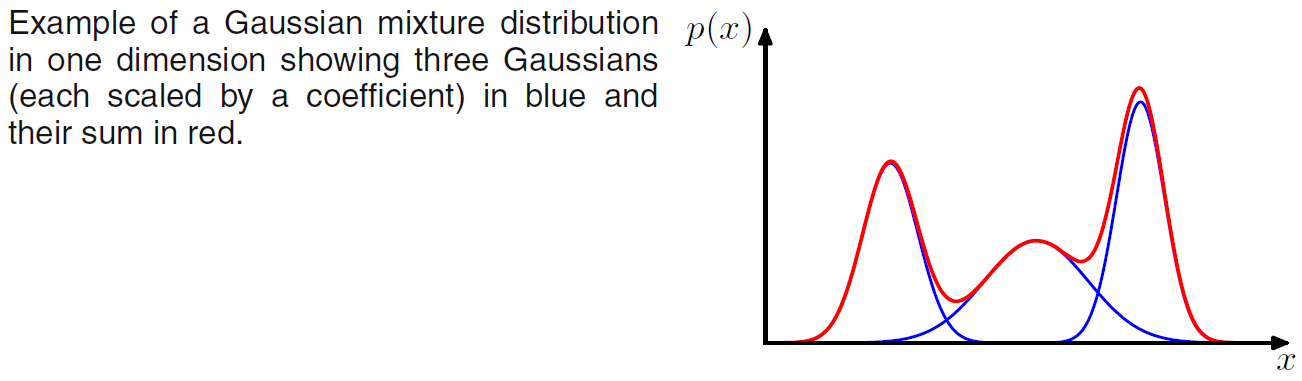
\includegraphics[width=17cm]{fig1.png}
\caption{Example of a Gaussian mixture distribution}
\label{fig:fig1}
\end{figure}

Such superpositions, formed by taking linear combinations of more basic distributions such as Gaussians, can be formulated as probabilistic models known as \emph{mixture distributions}. In Figure \ref{fig:fig1} we see that a linear combination of Gaussians can give rise to very complex densities. By using a sufficient number of Gaussians, and by adjusting their means and covariances as well as the coefficients in the linear combination, almost any continuous density can be approximated to arbitrary accuracy.

We therefore consider a superposition of $K$ Gaussian densities of the form
\begin{equation}\label{equ:mixture}
p(\mathbf x)=\sum_{k=1}^K\pi_k\mathcal N(\mathbf x|\boldsymbol\mu_k,\boldsymbol\Sigma_k)
\end{equation}
which is called a mixture of Gaussians. Each Gaussian density  $\mathcal N(\mathbf x|\boldsymbol\mu_k,\boldsymbol\Sigma_k)$ is called a component of the mixture and has its own mean $\boldsymbol\mu_k$ and covariance $\boldsymbol\Sigma_k$.

The parameters $\pi_k$ in (\ref{equ:mixture}) are called \emph{mixing coefficients}. If we integrate both sides of (\ref{equ:mixture}) with respect to $\mathbf x$, and note that both $p(\mathbf x)$ and the individual Gaussian
components are normalized, we obtain
\begin{equation}\label{equ:sum}
\sum_{k=1}^{K}\pi_k=1.
\end{equation}
Also, the requirement that $p(\mathbf x)\geq 0$, together with $\mathcal N(\mathbf x|\mu_k,\Sigma_k)\geq 0$, implies $\pi_k\geq 0$ for all $k$. Combining this with condition (\ref{equ:sum}) we obtain
\begin{equation}
0\leq\pi_k\leq 1.
\end{equation}

We therefore see that the mixing coefficients satisfy the requirements to be probabilities.

From the sum and product rules, the marginal density is given by

\begin{equation}
p(\mathbf x)=\sum_{k=1}^K p(k)p(\mathbf x|k)
\end{equation}
which is equivalent to (\ref{equ:mixture}) in which we can view $\pi_k=p(k)$ as the prior probability of picking the $k^{th}$ component, and the density $\mathcal N(\mathbf x|\boldsymbol\mu_k,\boldsymbol\Sigma_k)= p(\mathbf x|k)$ as the probability of $\mathbf x$ conditioned on $k$. From Bayes' theorem these are given by
\begin{equation}
\gamma_k(\mathbf x)=p(k|\mathbf x)=\frac{p(k)p(\mathbf x|k)}{\sum_lp(l)p(\mathbf x|l)}=\frac{\pi_k\mathcal N(\mathbf x|\boldsymbol\mu_k,\boldsymbol\Sigma_k)}{\boldsymbol\sum_l\pi_k\mathcal N(\mathbf x|\boldsymbol\mu_l,\boldsymbol\Sigma_l)}.
\end{equation}
The form of the Gaussian mixture distribution is governed by the parameters $\pi$, $\boldsymbol\mu$ and $\boldsymbol\Sigma$, where we have used the notation $\boldsymbol\pi=\{\pi_1,...,\pi_K\}$, $\boldsymbol\mu=\{\boldsymbol\mu_1,...,\boldsymbol\mu_k\}$ and $\boldsymbol\Sigma=\{\boldsymbol\Sigma_1,...,\boldsymbol\Sigma_K\}$. One way to set the values of there parameters is to use maximum likelihood. From (\ref{equ:mixture}) the log of the likelihood function is given by 
\begin{equation}
\ln p(\mathbf X|\boldsymbol\pi,\boldsymbol\mu,\boldsymbol\Sigma)=\sum_{n=1}^N\ln\{\sum_{k=1}^K\pi_k\mathcal N(\mathbf x_n|\boldsymbol\mu_k,\boldsymbol\Sigma_k\}
\end{equation}
where $X = \{\mathbf x_1,...,\mathbf x_N\}$. One approach to maximizing the likelihood function is to use iterative numerical optimization techniques. Alternatively we can employ a powerful framework called expectation maximization (EM).

\subsubsection{About Latent Variables}
We now turn to a formulation of Gaussian mixtures in terms of discrete \emph{latent} variables. This will provide us with a deeper insight into this important distribution, and will also serve to motivate the expectation-maximization (EM) algorithm.

Recall from (\ref{equ:mixture}) that the Gaussian mixture distribution can be written as a linear superposition of Gaussians in the form 
\begin{equation}\label{equ:form3}
p(\mathbf x)=\sum_{k=1}^K\pi_k\mathcal N(\mathbf x|\boldsymbol\mu_k,\boldsymbol\Sigma_k)
\end{equation}
Let us introduce a $K$-dimensional binary random variable $\mathbf z$ having a 1-of-$K$ representation in which a particular element $z_k$ is equal to 1 and all other elements are equal to 0. The values of $z_k$ therefore satisfy $z_k\in\{0,1\}$ and $\Sigma_k z_k=1$, and we see that there are $K$ possible states for the vector $\mathbf z$ according to which element is nonzero. We shall define the joint distribution $p(\mathbf x, \mathbf z)$ in terms of a marginal distribution $p(\mathbf z)$ and a conditional distribution $p(\mathbf x|\mathbf z)$. The marginal distribution over $\mathbf z$ is specified in terms of the mixing coefficients $\pi_k$, such that
\begin{equation}
p(z_k=1)=\pi_k
\end{equation}
where the parameters $\{\pi_k\}$ must satisfy
\begin{equation}
0\leq\pi_k\leq 1
\end{equation}
together with 
\begin{equation}
\sum_{k=1}^K\pi_k=1
\end{equation}
in order to be valid probabilities. Because $\mathbf z$ uses a 1-of-$K$ representation, we can also write this distribution in the form
\begin{equation}
p(\mathbf z)=\prod_{k=1}^K\pi_k^{z_k}.
\end{equation}
Similarly, the conditional distribution of $\mathbf x$ given a particular value for $\mathbf z$ is a Gaussian
\begin{equation}\label{equ:form1}
p(\mathbf x|z_k=1)=\mathcal(\mathbf x|\boldsymbol\mu_k,\boldsymbol\Sigma_k)
\end{equation}
which can also be written in the form
\begin{equation}\label{equ:form2}
p(\mathbf x|\mathbf z)=\prod^K_{k=1}p\mathcal(\mathbf x|\boldsymbol\mu_k,\boldsymbol\Sigma_k)^{z_k}.
\end{equation}
The joint distribution is given by $p(\mathbf z)p(\mathbf x|\mathbf z)$, and the marginal distribution of $\mathbf x$ is then obtained by summing the joint distribution over all possible states of $\mathbf z$ to give
\begin{equation}
p(\mathbf x)=\sum_{\mathbf z}p(\mathbf z)p(\mathbf x|\mathbf z)=\sum_{k=1}^K\pi_k\mathcal N(\mathbf x|\boldsymbol\mu_k,\boldsymbol\Sigma_k)
\end{equation}
where we have made use of (\ref{equ:form1}) and (\ref{equ:form2}). Thus the marginal distribution of $\mathbf x$ is a Gaussian mixture of the form (\ref{equ:form3}). If we have several observations $\mathbf{x_1,...,x_N}$, then, because we have represented the marginal distribution in the form $p(\mathbf x)=\sum_{\mathbf z}p(\mathbf x,\mathbf z)$, it follows that for every observed data point $\mathbf x_n$ there is a corresponding latent variable $\mathbf z_n$.

We have therefore found an equivalent formulation of the Gaussian mixture involving an explicit latent variable. It might seem that we have not gained much by doing so. However, we are now able to work with the joint distribution $p(\mathbf x, \mathbf z)$ instead of the marginal distribution $p(\mathbf x)$, and this will lead to significant simplifications, most notably through the introduction of the expectation-maximization (EM) algorithm.

Another quantity that will play an important role is the conditional probability of $\mathbf z$ given $\mathbf x$. We shall use $\gamma(z_k)$to denote $p(z_k=1|\mathbf x)$, whose value can be found using Bayes’ theorem

\begin{equation}
\gamma(z_k)=p(z_k=1|\mathbf x)=\frac{p(z_k=1)p(\mathbf x|z_k=1)}{\sum_{j=1}^Kp(z_j=1)p(\mathbf x|z_j=1)}=\frac{\pi_k\mathcal N(\mathbf x|\boldsymbol\mu_k,\boldsymbol\Sigma_k)}{\sum_{j=1}^K\pi_j\mathcal N(\mathbf x|\boldsymbol\mu_j,\boldsymbol\Sigma_j)}
\end{equation}
We shall view $\pi_k$ as the prior probability of $z_k=1$, and the quantity $\gamma(z_k)$ as the corresponding posterior probability once we have observed $\mathbf x$. As we shall see later, $\gamma(z_k)$ can also be viewed as the responsibility that component $k$ takes for ‘explaining’ the observation $\mathbf x$.




\subsection{EM for Gaussian Mixtures}
Initially, we shall motivate the EM algorithm by giving a relatively informal treatment in the context of the Gaussian mixture model.

Let us begin by writing down the conditions that must be satisfied at a maximum of the likelihood function. Setting the derivatives of $\ln p(\mathbf X|\boldsymbol\pi,\boldsymbol\mu,\boldsymbol\Sigma)$ with respect to the means $\boldsymbol\mu_k$ of the Gaussian components to zero, we obtain
\begin{equation}
0=-\sum_{n=1}^n\frac{\pi_k\mathcal N(\mathbf x_n|\boldsymbol\mu_k,\boldsymbol\Sigma_k)}{\underbrace{\sum_j\pi_j\mathcal N(\mathbf x_n|\boldsymbol\mu_j,\boldsymbol\Sigma_j)}_{\gamma(z_{nk})}}\sum_k(\mathbf x_n-\boldsymbol\mu_k)
\end{equation}

Multiplying by $\boldsymbol\Sigma_k^{-1}$ (which we assume to be nonsingular) and rearranging we obtain
\begin{equation}
\boldsymbol\mu_k=\frac{1}{N_k}\sum_{n=1}^N\gamma(z_{nk})\mathbf x_n
\end{equation}
where we have defined
\begin{equation}
 N_k=\sum_{n=1}^N\gamma(z_{nk}).
  \end{equation} 

We can interpret $N_k$ as the effective number of points assigned to cluster $k$. Note carefully the form of this solution. We see that the mean $\boldsymbol\mu_k$ for the $k^{th}$ Gaussian component is obtained by taking a weighted mean of all of the points in the data set, in which the weighting factor for data point $\mathbf x_n$ is given by the posterior probability $\gamma(z_{nk})$ that component $k$ was responsible for generating $\mathbf x_n$.

If we set the derivative of $\ln(\mathbf X|\boldsymbol\pi,\boldsymbol\mu,\boldsymbol\Sigma)$ with respect to $\boldsymbol\Sigma_k$ to zero, and follow a similar line of reasoning, making use of the result for the maximum likelihood for the covariance matrix of a single Gaussian, we obtain
\begin{equation}
\boldsymbol\Sigma_k=\frac{1}{N_k}\sum^N_{n=1}\gamma(z_{nk})(\mathbf x_n-\boldsymbol\mu_k)(\mathbf x_n-\boldsymbol\mu_k)^{\mathrm T}
\end{equation}
which has the same form as the corresponding result for a single Gaussian fitted to the data set, but again with each data point weighted by the corresponding posterior
probability and with the denominator given by the effective number of points associated with the corresponding component.

Finally, we maximize $\ln p(\mathbf X|\boldsymbol\pi,\boldsymbol\mu,\boldsymbol\Sigma)$ with respect to the mixing coefficients $\pi_k$. Here we must take account of the constraint $\sum_{k=1}^K\pi_k=1$. This can be achieved using a Lagrange multiplier and maximizing the following quantity
\begin{equation}
\ln p(\mathbf X|\boldsymbol\pi,\boldsymbol\mu,\boldsymbol\Sigma)+\lambda(\sum_{k=1}^K\pi_k-1)
\end{equation}
which gives
\begin{equation}
0=\sum_{n=1}^N\frac{\mathcal N(\mathbf x_n|\boldsymbol\mu_k,\boldsymbol\Sigma_k)}{\sum_j\pi_j\mathcal N(\mathbf x_n|\boldsymbol\mu_j,\boldsymbol\Sigma_j)}
\end{equation}
where again we see the appearance of the responsibilities. If we now multiply both sides by $\pi_k$ and sum over $k$ making use of the constraint $\sum_{k=1}^K\pi_k=1$, we find $\lambda=-N$. Using this to eliminate $\lambda$ and rearranging we obtain
\begin{equation}
\pi_k=\frac{N_k}{N}
\end{equation}
so that the mixing coefficient for the $k^{th}$ component is given by the average responsibility which that component takes for explaining the data points.
\subsection{EM Algorithm}
Given a Gaussian mixture model, the goal is to maximize the likelihood function with respect to the parameters (comprising the means and covariances of the components and the mixing coefficients).
\begin{enumerate}
	\item Initialize the means $\boldsymbol\mu_k$, covariances $\boldsymbol\Sigma_k$ and mixing coefficients $\pi_k$, and evaluate the initial value of the log likelihood.
	\item \textbf{E step}. Evaluate the responsibilities using the current parameter values
	\begin{equation}
	\gamma(z_{nk})=\frac{\pi_k\mathcal N(\mathbf x_n|\boldsymbol\mu_k,\boldsymbol\Sigma_k)}{\sum_{j=1}^K\pi_j\mathcal N(\mathbf x_n|\boldsymbol\mu_j,\boldsymbol\Sigma_j)}
	\end{equation}
	\item \textbf{M step}. Re-estimate the parameters using the current responsibilities
	\begin{gather}
	\boldsymbol\mu_k^{new}=\frac{1}{N_k}\sum_{n=1}^N\gamma(z_{nk})\mathbf x_n\\
	\boldsymbol\Sigma_k^{new}=\frac{1}{N_k}\sum_{n=1}^N\gamma(z_{nk})(\mathbf x_n-\boldsymbol\mu_k^{new})(\mathbf x_n-\boldsymbol\mu_k^{new})^{\mathrm T}\\
	\pi_k^{new}=\frac{N_k}{N}
	\end{gather}
	where 
	\begin{equation}
	N_k=\sum_{n=1}^N\gamma(z_{nk}).
	\end{equation}
	\item Evaluate the log likelihood
	\begin{equation}
	\ln p(\mathbf X|\boldsymbol\mu,\boldsymbol\Sigma,\boldsymbol\pi)=\sum_{n=1}^N\ln \{\sum_{k=1}^K\pi_k\mathcal N(\mathbf x_n|\boldsymbol\mu_k,\boldsymbol\Sigma_k\}
	\end{equation}
	and check for convergence of either the parameters or the log likelihood. If the convergence criterion is not satisfied return to step 2.
	
\end{enumerate}
\section{Tasks}
\begin{itemize}
	\item Assume that score vectors of teams in the same class are normally distributed, we can thus adopt the Gaussian mixture model. Please classify the teams into 3 classes by using EM algorithm. If necessary, you can refer to page 430-439 in the book \textcolor{blue}{\texttt{Pattern Recognition and Machine Learning.pdf}} and the website \textcolor{	orange}{\url{https://blog.csdn.net/jinping_shi/article/details/59613054}} which is a Chinese translation.
	\item You should show the values of these parameters: $\boldsymbol\gamma$, $\boldsymbol\mu$ and $\boldsymbol\Sigma$. If necessary, you can plot the clustering results. \textcolor{blue}{Note that $\boldsymbol\gamma$ is essential for classifying.}
	\item Please submit a file named \textcolor{orange}{\texttt{E13\_YourNumber.pdf}} and send it to \textcolor{orange}{\texttt{ai\_201901@foxmail.com}}
\end{itemize}
\section{Codes and Results}
\subsection{Code}
\begin{lstlisting}
#!/usr/bin/env python
# coding: utf-8

# In[1]:


# coding: utf-8
import numpy as np
import matplotlib.pyplot as plt


# In[2]:


def loadData(filename):
    """从文件中读取数据。"""
    dataSet = []
    id2country = []  # 将索引对应到国家名
    with open(filename) as fr:
        for i, line in enumerate(fr.readlines()):
            curLine = line.strip().split(' ')
            fltLine = list(map(int, curLine[1:]))  # 去掉第一列国家名
            dataSet.append(fltLine)
            id2country.append(curLine[0])
    return dataSet, id2country


# In[3]:


def prob(x, mu, sigma):
    """高斯分布的概率密度函数。"""
    n = np.shape(x)[1]
    expOn = float(-0.5 * (x - mu) * (sigma.I) * ((x - mu).T))
    divBy = pow(2 * np.pi, n / 2) * pow(np.linalg.det(sigma), 0.5)
    return pow(np.e, expOn) / divBy


# In[4]:


def EM(dataMat, maxIter=50):
    m, n = np.shape(dataMat)
    # 1.初始化各高斯混合成分参数
    alpha = [1/3, 1/3, 1/3]                                  # 初始化 alpha
    mu = [dataMat[1, :], dataMat[13, :], dataMat[11, :]]           # 初始化mu
    sigma = [np.mat((np.eye(7, dtype=float))) for x in range(3)]  # 初始化协方差矩阵
    gamma = np.mat(np.zeros((m, 3)))
    
    for i in range(maxIter):
        for j in range(m):
            sumAlphaMulP = 0
            for k in range(3):
                gamma[j, k] = alpha[k] * prob(dataMat[j, :], mu[k], sigma[k]) # 4.计算混合成分生成的后验概率,即gamma
                sumAlphaMulP += gamma[j, k]
            for k in range(3):
                gamma[j, k] /= sumAlphaMulP
        sumGamma = np.sum(gamma, axis=0)

        for k in range(3):
            mu[k] = np.mat(np.zeros((1, n)))
            sigma[k] = np.mat(np.zeros((n, n)))
            for j in range(m):
                mu[k] += gamma[j, k] * dataMat[j, :]
            mu[k] /= sumGamma[0, k] #  7.计算新均值向量
            for j in range(m):
                sigma[k] += gamma[j, k] * (dataMat[j, :] - mu[k]).T *(dataMat[j, :] - mu[k])
            sigma[k] /= sumGamma[0, k]  # 8. 计算新的协方差矩阵
            alpha[k] = sumGamma[0, k] / m   # 9. 计算新混合系数
        
        for s in sigma:
            s += np.eye(7)
            
    print('gamma')
    [print(g) for g in gamma]
    print('\nmu')
    [print(m) for m in mu]
    print('\nsigma')
    [print(s) for s in sigma]
    
    return gamma


# In[5]:


def initCentroids(dataMat, k):
    """Init centroids with random samples."""
    numSamples, dim = dataMat.shape
    centroids = np.zeros((k, dim))
    for i in range(k):
        index = int(np.random.uniform(0, numSamples))
        centroids[i, :] = dataMat[index, :]
    return centroids


# In[6]:


def gaussianCluster(dataMat):
    """进行聚类。"""
    m, n = np.shape(dataMat)
    centroids = initCentroids(dataMat, m)  ## step 1: init centroids
    clusterAssign = np.mat(np.zeros((m, 2)))
    gamma = EM(dataMat)
    for i in range(m):
        # amx返回矩阵最大值,argmax返回矩阵最大值所在下标
        clusterAssign[i, :] = np.argmax(gamma[i, :]), np.amax(gamma[i, :])  # 15.确定x的簇标记lambda
        ## step 4: update centroids
    for j in range(m):
        pointsInCluster = dataMat[np.nonzero(clusterAssign[:, 0].A == j)[0]]
        centroids[j, :] = np.mean(pointsInCluster, axis=0)  # 计算出均值向量
    return centroids, clusterAssign


# In[7]:


dataMat, id2country = loadData('football.txt')
dataMat = np.mat(dataMat)
centroids, clusterAssign = gaussianCluster(dataMat)


# In[8]:


result = ([], [], [])
for i, assign in enumerate(clusterAssign):
    result[int(assign[0, 0])].append(id2country[i])
print('\n-------------------------------------------\n')
print('First-class:', result[0])
print('Second-class:', result[1])
print('Third-class:', result[2])


# In[ ]:





\end{lstlisting}


\subsection{Results}
\begin{lstlisting}[language={}]
gamma
[[1.94167338e-114 1.25382308e-012 1.00000000e+000]]
[[1.00000000e+000 1.30157637e-090 6.99254748e-192]]
[[1.00000000e+000 1.77308433e-091 3.22118568e-308]]
[[1.00000000e+000 2.86831156e-033 3.89329040e-153]]
[[4.68941135e-103 1.00000000e+000 9.29410695e-122]]
[[1.73360486e-117 2.63382865e-004 9.99736617e-001]]
[[8.07501018e-70 1.52126772e-04 9.99847873e-01]]
[[1.73742960e-121 9.99999999e-001 9.91726551e-010]]
[[6.80507222e-64 1.00000000e+00 3.09330574e-23]]
[[2.99372863e-167 4.28991995e-061 1.00000000e+000]]
[[3.25570891e-236 7.31233936e-046 1.00000000e+000]]
[[1.25721563e-166 9.78317131e-042 1.00000000e+000]]
[[5.72371065e-127 1.00000000e+000 6.74033915e-028]]
[[1.13539296e-97 1.00000000e+00 3.40151214e-35]]
[[6.94426982e-210 5.86062654e-050 1.00000000e+000]]
[[1.00000000e+000 2.57084628e-074 2.29152462e-282]]

mu
[[21.5  21.25 28.5  20.5   5.25  2.75  3.25]]
[[39.60086419 38.40065967 47.99933524 41.19990029  8.39962848  7.99975071
   7.79983635]]
[[50.         48.5715611  45.71462493 44.28596869  7.28591355 12.4290124 
  11.14317249]]

sigma
[[ 2.725000e+01  3.875000e+00  0.000000e+00 -2.250000e+01 -4.875000e+00
  -1.250000e-01  8.875000e+00]
 [ 3.875000e+00  1.361875e+02 -1.625000e+00  6.875000e+00  5.937500e+00
   1.556250e+01  4.937500e+00]
 [ 0.000000e+00 -1.625000e+00  2.250000e+00  3.750000e+00  2.125000e+00
  -8.750000e-01 -3.750000e-01]
 [-2.250000e+01  6.875000e+00  3.750000e+00  3.325000e+01  1.162500e+01
  -8.750000e-01 -8.375000e+00]
 [-4.875000e+00  5.937500e+00  2.125000e+00  1.162500e+01  6.187500e+00
  -4.375000e-01 -2.062500e+00]
 [-1.250000e-01  1.556250e+01 -8.750000e-01 -8.750000e-01 -4.375000e-01
   3.187500e+00  5.625000e-01]
 [ 8.875000e+00  4.937500e+00 -3.750000e-01 -8.375000e+00 -2.062500e+00
   5.625000e-01  4.187500e+00]]
[[ 49.64494506  -0.63308678  -0.80684646  34.07613119  16.55476046
   -0.40255911 -12.48066475]
 [ -0.63308678  11.24631413  -3.20501105 -14.07962157 -13.76334855
   -1.60184591  -1.92210373]
 [ -0.80684646  -3.20501105  17.00398812   2.40059822   6.80240687
    8.00132936  -2.3984915 ]
 [ 34.07613119 -14.07962157   2.40059822  78.75365819  36.31742778
    1.2001994    1.4400767 ]
 [ 16.55476046 -13.76334855   6.80240687  36.31742778  26.44078121
    3.40083195  -0.71843719]
 [ -0.40255911  -1.60184591   8.00132936   1.2001994    3.40083195
    5.00041541  -1.19940939]
 [-12.48066475  -1.92210373  -2.3984915    1.4400767   -0.71843719
   -1.19940939   6.76032574]]
[[ 1.00000000e+00  3.78808699e-22  2.52540627e-22  1.89403069e-22
   1.01019058e-22  3.72504158e-22  9.47146495e-23]
 [ 3.78808699e-22  1.32439513e+01  8.16299251e+00  6.12224439e+00
  -2.44846776e+00  1.06118903e+01  3.06139095e+00]
 [ 2.52540627e-22  8.16299251e+00  2.54893112e+01  4.08042109e+00
   4.08073623e+00  1.46922298e+01  1.63256977e+01]
 [ 1.89403069e-22  6.12224439e+00  4.08042109e+00  2.54901593e+01
   1.63189594e+00  1.95911097e+01  1.36729295e+01]
 [ 1.01019058e-22 -2.44846776e+00  4.08073623e+00  1.63189594e+00
   9.48874928e+00  5.87641959e+00  4.81500277e+00]
 [ 3.72504158e-22  1.06118903e+01  1.46922298e+01  1.95911097e+01
   5.87641959e+00  3.03862236e+01  2.29377945e+01]
 [ 9.47146495e-23  3.06139095e+00  1.63256977e+01  1.36729295e+01
   4.81500277e+00  2.29377945e+01  2.96935612e+01]]
   
-------------------------------------------

First-class: ['Japan', 'South_Korea', 'Iran', 'Australia']
Second-class: ['Saudi_Arabia', 'United_Arab_Emirates', 'Uzbekistan', 'Bahrain', 'North_Korea']
Third-class: ['China', 'Iraq', 'Qatar', 'Thailand', 'Vietnam', 'Oman', 'Indonesia']
\end{lstlisting}

%\clearpage
%\bibliography{E:/Papers/LiuLab}
%\bibliographystyle{apalike}
\end{document} 
%%% Local Variables:
%%% mode: latex
%%% TeX-master: t
%%% End:
